\chapter{Introduction}

\section{The Rise of Digital Identity Wallets and the Need for Secure, Private, Usable Solutions}
Digital credential wallets, the digital analogue of their physical counterparts, are emerging as essential tools for identity verification in both online and offline contexts. Nations such as India, Singapore, South Korea, Estonia, and Norway have implemented nationwide digital identity systems, while the EU mandates wallets and digital credential issuance across member states by 2026, and the US advances pilots in 13 states.  These systems aim to streamline identity management by using interoperable wallets built on open standards, yet their success depends on resolving a fundamental trilemma: ensuring privacy, security, and usability. Consider the following scenarios

\begin{enumerate}\label{chap1_use_cases_kyc_socialmedia_age_and_health}
    \item \textbf{KYC/AML Bank Application}: Opening a bank account requires verifying citizenship, age, government issued credentials, and possibly financial standing (bank balances). Traditional KYC processes are slow and complex, with up to 68\% of users abandoning applications, with additional privacy risks of sharing and storing user personal information

    \item \textbf{Social Media Verification:} Accessing social media in Australia will soon require age (over 16) and citizenship verification. A frequent transaction that could leak a childs online movements 

    \item \textbf{Age and Health Status: } Interacting with a medical clinic often requires different criteria to be met, such as a vaccination status, age, and insurance status. Current processes require a user to show all information during the process. 
\end{enumerate}

Across these cases, users seek privacy; disclosing only essential information, while verifiers require security, such as authenticity and fraud resistance. Usability demands \emph{fast} verification of multiple, heterogeneous credentials. Yet, prior systems expose user data and fuel cybercrime, or privacy-preserving systems lack efficiency. The previous generation\footnote{We term the "previous generation" as credentials which compute presentation proofs using $\G_T$ points, as this Thesis shows, is significantly slower. We term "new generation" credential frameworks that compute proofs over $\G_1$  \cite{camenisch_anonymous_2016, tessaro_revisiting_2023, tomescu_utt_2022}, demonstrating remarkable efficiency improvements} of anonymous credential frameworks \cite{hutchison_signature_2004, hutchison_constant-size_2006, sako_short_2016}, deployed in Microsoft's U-Prove and IBM's Idemix \cite{camenisch_design_2002, dunkelman_formal_2016}, though innovative, met basic needs—verifying a single credential in 50ms—but fail to address the complex, multi-credential and sybil resistant demands of the next generation of identity systems. Verifying multiple credentials is either too slow, lacks a theoretical framework and security properties, or lacks efficient and private mechanisms for sybil resistance and revocation. These gaps are already driving discussions at the Internet Identity Workshop \cite{internet_identity_workshop_internet_2025} and looking for solutions with discussions on how the credential wallet will securely issue and verify credentials from multiple different issuers (government, private, credential oracles); how can an efficient sybil resistance mechanism be incorporated inside a credential wallet.

This thesis develops cryptographic primitives to enable digital credential wallets that are fast, private, and resilient to abuse, paving the way for advanced identity solutions that solve for the upcoming limitations that credential wallets will pose, and unlock new functionality for secure and private digital interactions.


\section{Anonymous Credentials}
Anonymous credential systems enable privacy-preserving authentication and access control, allowing users to prove specific attributes without revealing their full identity. Anonymous Credentials is the base building block of digital credential wallets, where users manage diverse credentials (e.g., passports, bank statements) to verify identity across scenarios like KYC or age verification. They fulfill two primary roles: ensuring holder authenticity like signature verification (e.g., proving knowledge of a secret key) and enforcing access control (e.g., demonstrating eligibility based on attributes like age $ > 21 $).

% https://eprint.iacr.org/2024/1874.pdf#page=22.70
Anonymous Credentials are a subset of Verifiable Credentials, defined by W3C  \cite{w3c_verifiable_2025}, as "tamper-evident credential whose authorship can be cryptographically verified", a Verifiable Presentation is a function of a VC which creates "A tamper-evident presentation of information encoded in such a way that authorship of the data can be trusted after a process of cryptographic verification." This Thesis focuses on private Verifiable Presentations that leverage zero-knowledge proofs to privately attest to the data within the Verifiable Credential. 

The Anonymous Credential framework involves three main actors: the \emph{user}, who owns the credential wallet with credentials, their attributes, and their signing/verification keys; the \emph{issuer}, who creates credentials; and the \emph{verifier}, who checks them. Credentials are authenticated data structures that cryptographically bind attributes, ensuring both hiding (privacy) and binding (security). These structures vary by issuance model and underlying cryptographic primitive. Credentials could be issued by a single-issuer as most are issued today, or to protect against malicious issuers, it could be threshold of issuers or even blockchain-based smart contracts. Credentials could be in the form of signatures or even data-structures in a cryptographic accumulator. The choice of cryptographic data structure dictates the proof system, the proof expressiveness, and the verification efficiency.

\begin{figure}
    \centering
    \scalebox{0.85}{ % Scale down the entire figure to 85%
        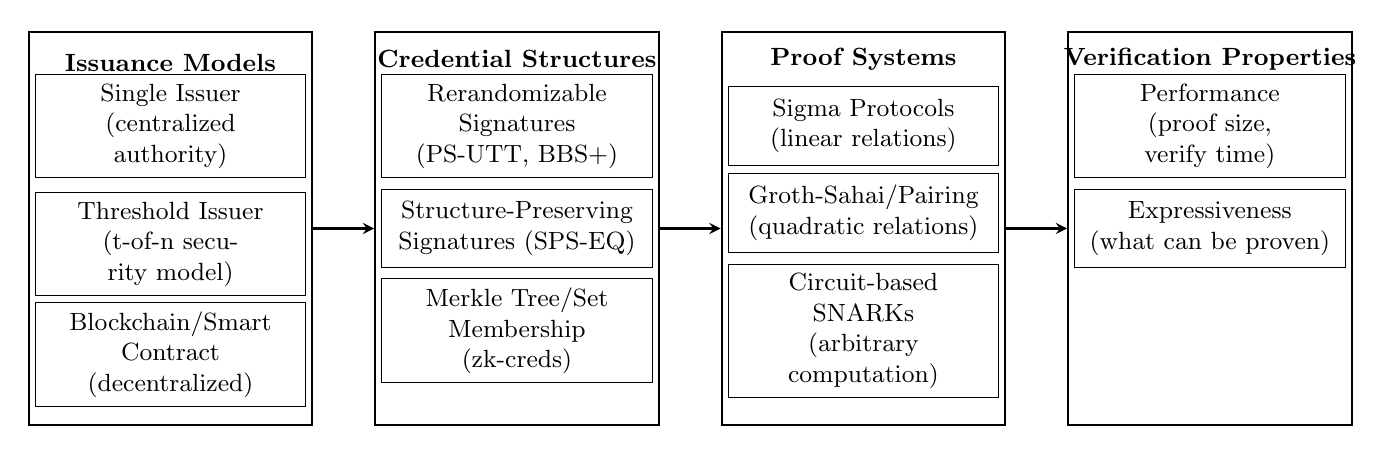
\begin{tikzpicture}[
            box/.style={
                rectangle,
                draw=black,
                thick,
                minimum width=3.6cm,
                minimum height=5cm,
            },
            title/.style={
                rectangle,
                draw=none,
                thick,
                minimum width=3.4cm,
                minimum height=0.8cm,
                align=center,
                font=\bfseries\small
            },
            item/.style={
                rectangle,
                draw=black,
                text width=3.2cm,
                minimum height=1cm,
                align=center,
                font=\small
            },
            arrow/.style={->, >=stealth, thick}
        ]
        
        % Outer boxes with 0.5cm added between them
        \node[box] (box1) at (0,0) {};
        \node[box] (box2) at (4.4,0) {}; % Increased from 3.9 to 4.4 (+0.5cm)
        \node[box] (box3) at (8.8,0) {}; % Increased from 7.8 to 8.8 (+0.5cm)
        \node[box] (box4) at (13.2,0) {}; % Increased from 11.7 to 13.2 (+0.5cm)
        
        % Box titles
        \node[title] (t1) at (0,2.1) {Issuance Models};
        \node[title] (t2) at (4.4,2.15) {Credential Structures}; % Updated position
        \node[title] (t3) at (8.8,2.15) {Proof Systems}; % Updated position
        \node[title] (t4) at (13.2,2.15) {Verification Properties}; % Updated position
        
        % Connecting arrows
        \draw[arrow] (box1.east) -- (box2.west);
        \draw[arrow] (box2.east) -- (box3.west);
        \draw[arrow] (box3.east) -- (box4.west);
        
        % Items for box 1 - preserving user's vertical position adjustments
        \node[item] (i11) at (0,1.3) {Single Issuer\\(centralized authority)};
        \node[item] (i12) at (0,-0.2) {Threshold Issuer\\(t-of-n security model)};
        \node[item] (i13) at (0,-1.6) {Blockchain/Smart Contract\\(decentralized)};
        
        % Items for box 2
        \node[item] (i21) at (4.4,1.3) {Rerandomizable Signatures\\(PS-UTT, BBS+)}; % Updated position
        \node[item] (i22) at (4.4,0) {Structure-Preserving\\Signatures (SPS-EQ)}; % Updated position
        \node[item] (i23) at (4.4,-1.3) {Merkle Tree/Set Membership\\(zk-creds)}; % Updated position
        
        % Items for box 3 - preserving user's vertical position adjustments
        \node[item] (i31) at (8.8,1.3) {Sigma Protocols\\(linear relations)}; % Updated position
        \node[item] (i32) at (8.8,0.2) {Groth-Sahai/Pairing\\(quadratic relations)}; % Updated position
        \node[item] (i33) at (8.8,-1.3) {Circuit-based SNARKs\\(arbitrary computation)}; % Updated position
        
        % Items for box 4
        \node[item] (i41) at (13.2,1.3) {Performance\\(proof size, verify time)}; % Updated position
        \node[item] (i42) at (13.2,0) {Expressiveness\\(what can be proven)}; % Updated position
        
        \end{tikzpicture}
    }
    \caption[Anonymous Credential Framework Diagram]{Anonymous Credential Framework. The Issuance Model determines the Credential Type. The Credential Structure and underlying commitment determines the Proof System and Verification Properties}
    \label{fig:chap1_anon_cred_framework}
\end{figure}

Two core interactive processes govern anonymous credentials. In the \emph{obtain/issue} phase, users commit attributes, and issuers sign them, often blindly to preserve a user's privacy. In the \emph{show/verify} phase, users generate a Verifiable Presentation to meet dynamic verification requirements (e.g., proving $ \text{age} > 16 $ without disclosing birthdate). Verifiers check these proofs for validity. Proof systems, such as Sigma protocols, Groth-Sahai, pairing-based methods or zk-SNARKS, balance expressiveness (e.g., proving complex predicates) with efficiency.

Security hinges on two main properties: \emph{unforgeability}, ensured by the binding nature of commitments and soundness of proofs, and \emph{anonymity}, achieved through hiding commitments, homomorphism of randomizing actions and the zero-knowledge property of zero-knowledge proofs, preventing linkability across verifications. However, designing systems that scale to multi-credential wallets, resist abuse, and perform efficiently involves trade-offs in privacy, efficiency, and expressiveness. These challenges highlight the need for careful selection of combining the fastest cryptographic primitives or optimizing the existing primitives to minimize computational overhead, selecting the most expressive schemes to enable the use-case functionality that is needed for next-generation identity systems.
This Thesis addresses each of these and demonstrates our state-of-the-art primitives via qualitative and quantitiave analysis. 



\section{Limitations of Previous Approaches}
The Trilemma between Privacy, Security, and Usability presents ongoing challenges and limitations. Privacy-preserving systems aim for \emph{Accountable Privacy} within acceptable usability limits. The Trilemma tension arises due to the paradoxical nature of each property. Increasing Privacy and Security comes at the cost of Usability, and vice versa. The Gap Analysis often articulates the \emph{cost of privacy} system architects must weigh when considering privacy-preserving primitives.

\subsection{Limitation 1: Fast Anonymous Credentials (close to ECDSA)}\label{subsec:chap1_limitation1}

Anonymous credentials fundamentally operate slower than traditional signature schemes like ECDSA which has long limited their adoption. Benchmarks \cite{habib_evaluation_2016} have shown $\mathsf{Show + Verify}$ time for Anonymous Credential systems IBM's Idemix to be $(110ms, 220ms, 450ms)$ for 1,2,3 credentials, Microsoft's U-Prove to be $(180ms, 460ms, 600ms)$ for 1,2,3 credentials respectively, IRMA \cite{fischer-hubner_towards_2013} at $1300ms$ and zk-creds at $465ms$ \cite{rosenberg_zk-creds_2022}. Consider Alice approaching a turnstyle for the train needing to verify her transport ticket and student status. Non-private signatures would sign and verify under $1ms$, whereas current anonymous credentials benchmarks are beyond the $100ms$ rule applied by user experience experts \cite{jakob_nielsen_powers_2009} and threshold for revenue loss due to webpage loads at Google and Amazon \cite{linden_geeking_2006}. The consequence is users and system architects prioritizing efficiency over privacy and using non-private methods of authentication. 


\subsection{Limitation 2: Security Against Malicious Issuers}
Most Anonymous Credential systems deployed today assume honest-but-curious issuers rather than actively malicious ones; such systems claim strong security and privacy guarantees but fail to recognize the threat from maliciously generated signing and verification keys, which could allow a signer to secretly embed tracking or de-anonymizing algebraic structure into the credential. This would undermine the systems privacy guarantees and prevent widespread adoption. 


\subsection{Limitation 3: Efficient Expressive Proofs}
Current Anonymous Credential Benchmarks show computationally expensive expressive proof evaluation. \cite{habib_evaluation_2016} demonstrates Idemix running Show+Verify for a credential with 5 attributes including string equality (120ms) and separately "date greater than" (310ms). zk-creds \cite{rosenberg_zk-creds_2022} demonstrates two use-cases, accessing a website proving over 18 with Show+Verify of 148ms best case or 602ms worst case, and verifying a credential in-person and selectively disclosing age and photo being 103ms best case and 602ms worst case\footnote{worst case scenarios come from Merkle Tree proof update}. All of which are over the $100ms$ threshold discussed in Limitation 1 \ref{subsec:chap1_limitation1}, hindering realistic uptake of new technology. 


\subsection{Limitation 4: Secure and Efficient Verification of Multiple Credentials}
There has been some consideration of the need to securely verify multiple credentials simultaneously while proving that such credentials come from the same user. Credential wallets provide the perfect use-case, our use-cases \ref{chap1_use_cases_kyc_socialmedia_age_and_health} are prototypical but it is easy to see where this functionality can be extended to, online application KYC requirements show 68\% of consumers abandon their application because of delays \cite{signicat_battle_2022}, especially with content credentials \cite{c2paorg_content_2024} producing a credential for each transaction, photo, or message sent from a device. \cite{dunkelman_formal_2016} includes the functionality in security proofs, but not as an explicit property; furthermore, while it is a theoretical property, no schemes attempt to clearly present benchmarks on practical feasibility. 


\subsection{Limitation 5: Efficient Nullifiers for Sybil Resistance}
Nullifiers are used in privacy-preserving systems to prove sybil resistance while retaining anonymity. A user generates a nullifier from their key and some input and wants to keep their key secret to uphold anonymity (and prevent tracking through system use). In payment systems, the input might be a coin's serial number \cite{ben_sasson_zerocash_2014, tomescu_utt_2022}, and Identity Systems might use the credential context, e.g., "passport" to ensure a user has only 1 passport, or "2025vote" to enforce sybil-resistant voting. Zerocash \cite{ben_sasson_zerocash_2014} and PLUME \cite{gupta_plume_2022} leverage zk-SNARKS $(50+ms)$ while \cite{tomescu_utt_2022} leverage pairing constructions $(12.38ms)$, all with computational overhead (possibly more than one nullifier can be used in a presentation), which combined with credential verification and expressive proofs will extend Show+Verify times beyond acceptable limits, rendering the cost of privacy too high for practical use. 


\subsection{Limitation 6: Efficient Threshold Signatures for Threshold Issued Identity System}
Current threshold credential schemes for threshold-issued identity systems present with prohibitively slow operations or lack benchmark analysis to conclude otherwise. Threshold BBS+ was proposed \cite{doerner_threshold_2023} and initial benchmarks show signing times of 38 seconds \cite{dock_network_crypto_2025} though the scheme is without identifiable abort, its inclusion would be more expensive. tACT-based systems like S3ID \cite{rabaninejad_attribute-based_2024} show verification times that scale poorly with attribute count. Threshold implementations of SPS-EQ \cite{steinfeld_threshold_2023} may address efficiency, but they lack performance benchmarks. The performance gap, lack of evaluation metrics create and concrete implementations in an identity system create barriers to adoption. 


\subsection{Limitation 7: Understanding the (Empirical) Cost of Privacy}
Organizations wanting to adopt Anonymous Credential frameworks for integration to their identity systems lack empirical benchmarks across various schemes which would allow them to select a scheme based on its properties and empirical analysis. It's hard to understand the "cost" of privacy based on the literature and implementations available. Furthermore, IT departments benefit from experimenting with code to learn. Some academic implementations include code samples but often are built with different libraries, languages, and enhancements - it's difficult to assess and compare schemes in this environment. 


\section{Contributions}


\begin{figure}[!htb]
    \centering
    
   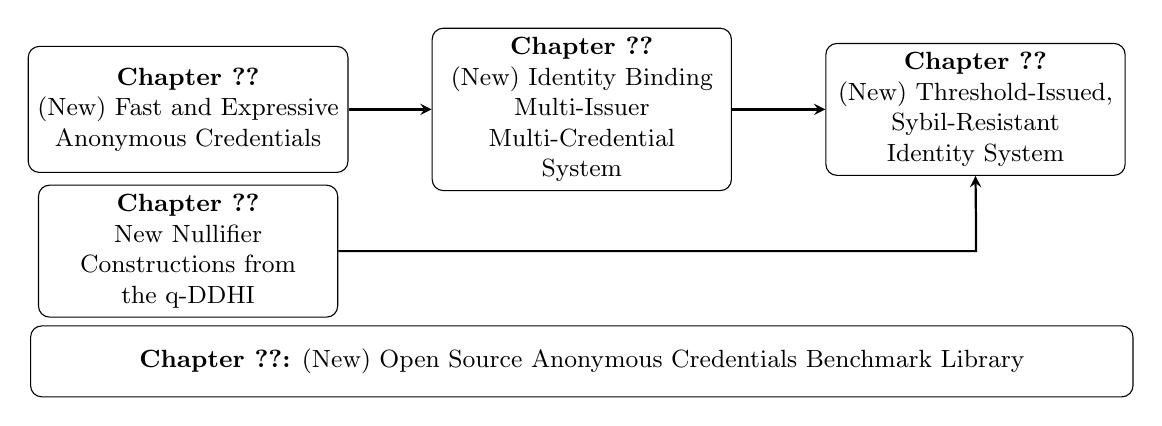
\begin{tikzpicture}[
    % Node styles with reduced sizes
    chapter/.style={
        draw,
        rounded corners,
        minimum width=3.8cm,         % Reduced from 4.5cm
        minimum height=1.6cm,        % Reduced from 2cm
        align=center,
        font=\small                  % Reduced font size
    },
    benchmark/.style={
        draw,
        rounded corners,
        minimum width=14cm,          % Reduced from 16.5cm
        minimum height=0.9cm,        % Reduced from 1.2cm
        align=center,
        font=\small                  % Reduced font size
    },
    % Arrow style
    arrow/.style={thick, ->, >=stealth}
    ]

    % Top row chapters - same horizontal positions but tighter
    \node[chapter] (ch2) at (0,0) {\textbf{Chapter \ref{chap2}}\\(New) Fast and Expressive\\Anonymous Credentials};
    
    \node[chapter] (ch3) at (5,0) {\textbf{Chapter \ref{chap3}}\\(New) Identity Binding\\Multi-Issuer\\Multi-Credential\\System};
    
    \node[chapter] (ch5) at (10,0) {\textbf{Chapter \ref{chap5}}\\(New) Threshold-Issued,\\Sybil-Resistant\\Identity System};
    
    % Bottom row - Chapter 4 with reduced vertical gap
    \node[chapter] (ch4) at (0,-1.8) {\textbf{Chapter \ref{chap4}}\\New Nullifier\\Constructions from\\the q-DDHI};
    
    % Chapter 6 with reduced vertical gap
    \node[benchmark] (ch6) at (5,-3.2) {\textbf{Chapter \ref{chap6}:} (New) Open Source Anonymous Credentials Benchmark Library};
    
    % Arrows connecting chapters
    \draw[arrow] (ch2) -- (ch3);
    \draw[arrow] (ch3) -- (ch5);
    
    % Draw arrow from Chapter 4 to Chapter 5's bottom edge
    \draw[arrow] (ch4.east) -- ++(8.1,0) -- ++(0,0.3) -- (ch5.south);
    
    \end{tikzpicture}
    
    \caption{Contribution Roadmap}
    \label{fig:chap1_contribution_roadmap}
\end{figure}


\subsection{Chapter \ref{chap2}: Fast and Expressive Anonymous Credentials from New Rerandomizable Signatures}
This chapter directly targets the security-privacy-usability trilemma by improving the base building block, the credential construction itself. I address \textbf{limitations 1, 2, and 3}, by constructing the most efficient Anonymous Credential for Verifiable Presentations (according to my research and benchmarks) by enhancing a variant \cite{tomescu_utt_2022} of the PS signature \cite{sako_short_2016} with Show+Verify time of 3.77ms for a credential with 10 attributes. I also provide empirical, fair benchmarks against the state-of-the-art schemes \cite{hutchison_constant-size_2006, camenisch_anonymous_2016, sako_short_2016, tomescu_utt_2022} using the same cryptography libraries and coding language to ensure comparison takes into account the cryptography itself. Additionally, I included security against malicious issuers by adapting the framework in \cite{fuchsbauer_structure-preserving_2019}, and proved my construction of Rerandomizable Signatures secure in the Anonymous Credential model from \cite{fuchsbauer_structure-preserving_2019}. I also demonstrate that the proof system, $\Sigma$-protocols, excels in satisfying the efficiency-expressive tradeoff. 


\subsection{Chapter \ref{chap3}: Identity Binding Multi Issuer Multi Credential Anonymous Credentials}
I address \textbf{limitation 4} in this chapter by tackling the challenge of verifying multiple credentials from different issuers while proving they belong to the same user, a key requirement for credential wallets. I create the \emph{Identity Binding} security property for such schemes. I address \textbf{limitation 7} by extensively benchmarking the use-case scenarios. I built a Multi-Issuer Multi-Credential System in Rust and benchmarked different scenarios. First, \emph{non-private} multi-credential usage for 16 unique credentials, 16 attributes each credential from unique issuers, cost just ~27ms (Verify). The \emph{cost of privacy} for (Show + Verify) was just 2.6x at ~72ms. I also show that credentials signed by a single issuer with our construction can use signature aggregation and reduce (Show + Verify) to just 31ms for the same (16 credentials with 16 attributes in each). This chapter proves that complex identity assertion requirements like KYC/AML, incorporating multiple credentials, can be extraordinarily efficient with credential wallets.


\subsection{Chapter \ref{chap4}: New Nullifier Constructions from the q-DDHI and Applications to Accountably Private Systems.}
In this chapter we resolve \textbf{limitation 5} by introducing fast, private nullifier constructions using the $q-$DDHI assumption and novel $\Sigma$-protocols. I first introduce a pairing-free (Non-Private) Dodis Yampolskiy (DY) \cite{hutchison_verifiable_2005} Verifiable Random Function (VRF) construction from the $q-$DDHI assumption (rather than $q$-DBDHI) that is 3x more efficient than the original, and because we remove pairings, we can use non-pairing curves e.g. Ed25519 for 6x speedup. This has applications broader than nullifier schemes. Next, I developed 3 x novel $\Sigma-$ protocols to privately prove the DY structure (in zero knowledge) from committed attributes and constructed deterministic and probabilistic nullifiers with applications to sybil resistance and revocation in privacy-preserving protocols. The deterministic nullifier is at least 5x faster than previous constructions \cite{tomescu_utt_2022}.

\subsection{Chapter \ref{chap5}: Threshold-Issued, Sybil-Resistant Private Identity System from Anonymous Credentials and Nullifiers}
This chapter constructs a Threshold-Issued, Sybil-Resistant identity system addressing \textbf{limitation 6}. We first demonstrate our base-building block, the Threshold Signature construction is extremely efficient as we compare against tACT a state-of-the-art system \cite{rabaninejad_attribute-based_2024}. We then construct a Sybil Resistant Identity System drawing on the work in  Chapters \ref{chap2}, \ref{chap3}, \ref{chap4} and show it's exponentially faster for end to end performance metrics \ref{chap5:sec_tsiris}.

\subsection{Chapter \ref{chap6}: Open Source Anonymous Credential Library}
To bridge the gap in standardized evaluations, we develop an open-source library benchmarking state-of-the-art credential schemes under consistent conditions. This resolves \textbf{limitation 7}, giving practitioners the tools to test different constructions and work with empirical data. This library also reveals practical efficiency gains from cryptography library functions like Multi-Scalar Multiplication, Miller-Loop Pairing computation.



